\chapter{Background}
\section{Bulk Synchronous Parallel} \label{sec:bsp}
Bulk Synchronous Parallel (BSP) is a bridging model introduced by L.G. Valiant in \cite{Valiant:1990:BMP:79173.79181}. A bridging model describes a conceptual understanding of
hardware for the purpose software development. The most basic of these models is the von Neumann architecture, which is still used as the basic understanding of sequential hardware in modern CPUs. In the wake of parallel computing, BSP was proposed to fulfil the same roll
for the understanding of parallel hardware. The model does not specify how any of the elements should be realised in hardware or software, since it's purpose is to provide a common ground for hardware and software developers. 
BSP fundamental principal is the separation of computation and communication. A computer modelled after BSP requires
\begin{enumerate}
	\item a set of components or execution units, performing the computational work of the algorithm.
	\item a router to convey information between the components.
	\item a facility to synchronize some or all of the components in steady intervals.
\end{enumerate}
Each component performs local computations and then shares it's results with
the other components via the rounter. The synchronization guarantees that all components completed computation and communication. The sequence of computation, communication and synchronization is called a superstep. One or more supersteps are used to implement an algorithm.
The model allows excluding components from synchronization, if the algorithm allows or requires it.

Although all computations are supposed to be local, BSP allows concurrent read and concurrent write access to a shared memory between the
components. But this is only allowed, if the underlying memory system guarantees coherent and consistent resolution of access conflicts.

\section{General Purpose GPU Compuing}
GPGPU computing utilizes GPUs for computations other that graphics. With CUDA, NVidia offers a C-based, proprietary language to write application for NVidia GPUs. GPUs are so called "many-core" processors, with thousands of compute units (CUDA cores). CUDA cores are clustered in Streaming Multiprocessors(SM), executing 32 threads concurrently. Code executed on a GPU is capsuled in a kernel. Figure \ref{gpu-hier} is an overview of the features detailed in the next sections. Nvidia also offers an assembler-like language called PTX, that is not architecture generation specific. \cite[4.1-4.2	]{cuda-man}

\subsection{Execution Model}
Threads is CUDA are hierarchically organized. Groups of up to 1024 threads are organized in a 3D block, called "Collaborative Thread Array" (CTA). The execution of one compute kernel consists of many CTAs, organized in a 3D grid. During a kernel execution, the CTAs are  scheduled to a SM in a non-deterministic fashion, based on available resources. Once a CTA is scheduled, it can not be pre-empted and executes until it is finished.  \cite[2.1 - 2.2]{cuda-man}

The threads inside a CTA are organized in groups of 32, called warp. All threads in a warp execute the same instruction stream. If the one or more threads in a warp have a branch in the CFG, all threads in the warp
execute the branch, but only the ones supposed to work create side-effects. The shared instruction stream continues if all threads finished a branch. \cite[4.1]{cuda-man}

A kernel usually consists of more CTAs than a GPU can execute concurrently. Non-deterministic scheduling on the GPU  prevents predictions on the CTA execution order, making CTA interaction
in a kernel a deadlock hazard. Therefore interaction of threads belonging to different CTAs are not allowed. The execution model allows threads inside the same CTA to interact using Shared Memory, which is located in the SM and private for each CTA. \cite[5]{cuda-man}

Kernels are executed in the order in which the kernel calls are issued by the application. CUDA streams allow concurrent  execution of multiple kernels and data movement, given the resources are available on the GPU. \cite[5]{cuda-man}

\subsection{Memory Model}
GPUs have a hierarchical memory model, with different address spaces. Table \ref{GPUMemTable} lists all available memories and their properties. For this work we will focus on global memory, as it is the only 
memory allowing modification by a kernel, which persist beyond the kernel completion boundary.
Host-Mapped memory falls in the same category as global, and for our purposes is treated as global memory. 

It is important to note, that CUDA only guarantees a consistent state of global memory, after the kernel completion 
boundary. There are no guarantees on global memory consistency during the execution of a kernel, which is another reason
CTA interaction at kernel run-time is not intended. \cite[B5-B7]{cuda-man}
\begin{figure}[t]
	\centering
	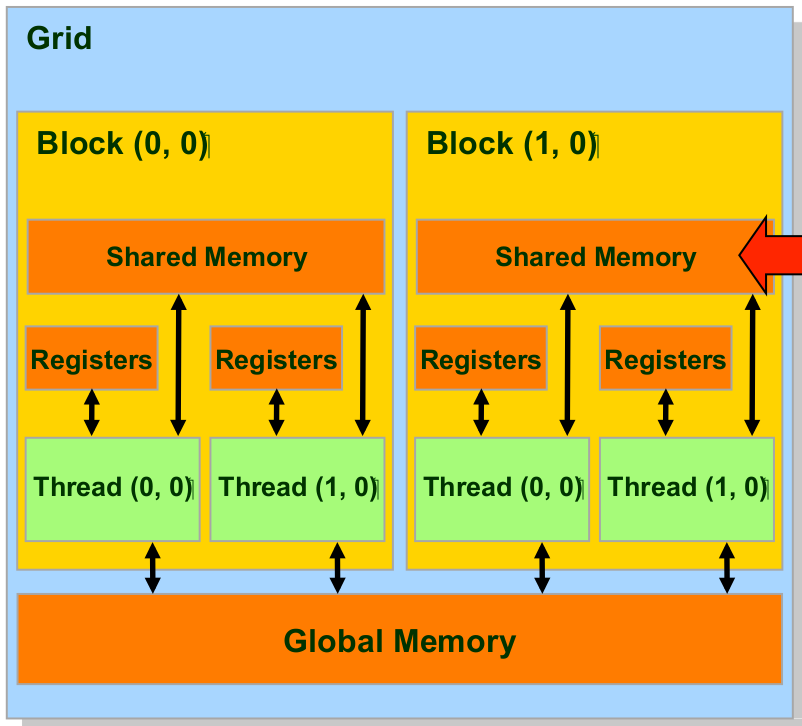
\includegraphics[width=0.6\textwidth]{gpu-arch}
	\caption{GPU thread and memory hierarchy. Image form \cite{}}
	\label{gpu-hier}
\end{figure}
\begin{table}
	\centering
	\begin{tabular}{|l|c|c|c|c|c|c|}
		\hline 
		\textbf{Memory} & \textbf{Scope} & \textbf{Access} & \textbf{Bandwidth} & \textbf{Latency} & \textbf{Capacity} & \textbf{Location} \\ 
		\hline
		\hline
		Register  & Thread & RAM & high & low & 32bit & SM \\ 
%		\hline 
		Shared  & CTA & RAM & high & low & < 48k & SM \\ 
%		\hline 
		Global  & Kernel & RAM & high & high & < 20GB & device \\ 
%		\hline 
		Texture/Constant & Kernel & ROM & high & high & < 20GB & device \\ 
%		\hline 
		Host-Mapped  & Kernel+CPU & RAM & low & high & > 20GB & host \\ 
		\hline 
	\end{tabular} 
	\caption{GPU Memory Types, move to Background chapter. \cite[2.3]{cuda-man}}
	\label{GPUMemTable}
\end{table}
\section{LLVM}
LLVM is a compiler project providing tools for full-stack compiler development. While originally written for C/C++, nowadays front-ends for many languages are provided and back-ends for many different architectures are available. The C/C++ compiler using the LLVM tool-chain is called Clang. Since 2015 Clang and the LLVM
tool-chain support CUDA code and can produce PTX files for GPU execution \cite{gpucc}.
LLVM uses an intermediate representation (IR) for code analysis and optimization 
(more on this in \ref{llvmir}). Code compiled with Clang is translated into IR and then further processed. \cite{Lattner:2004:LCF:977395.977673}

For this work, we will distinguish the tool-chain into three major components:
\begin{itemize}
	\item The \textbf{front-end} takes care of pre-processing, lexical, and syntactical analysis of the original code. Clang uses an Abstract Syntax Tree (AST) to represent the original code. This AST is accessible via an API and additional plug-ins can be added to the tool-chain. After the lexical and syntactical analysis are complete, the code is translated into IR. 
	\item The \textbf{optimizer} uses the IR to analyse and then transform the code. The IR is accessible with an API and allows the introduction of additional modules for analysis or transformation. These modules are called a "pass" (details in section \ref{llvmpass}).
	\item The \textbf{back-end} includes the linker and back-end architecture depended code generation. This part of the
	toolchain is not relevant for this work and is only mentioned for completeness.
\end{itemize}
This overview gives an sufficient understanding of the LLVM stack for this work and in the following sections
the concepts of IR and passes are explored in more depth.

\subsection{LLVM IR Program Representation} \label{llvmir}
LLVM's IR is a typed RISC instructions set with a load/store memory architecture. The IR is architecture agnostic and provides an infinite set of virtual, typed registers. The available primitive language-independent types are: (un)signed integer (8-64 bit), single and double precision floating point, and Boolean. Derived from these primitive types are the aggregate types pointers, arrays, structures, and functions. In LLVM it is possible to transform form any type into an arbitary other type, using the \verb|cast| instruction. \cite{Lattner:2004:LCF:977395.977673}

Any kind of pointer arithmetic and access to aggregate types is performed by the \verb|getelementptr| (\verb|gep|) instruction, which preserves type information, is machine and language independent, and returns a pointer. Using \verb|gep| allows the IR to keep load/store instructions clean and only use the direct address to access element.
\cite{Lattner:2004:LCF:977395.977673}

One important part of LLVM's code transformations are canonicalization and lowering, which happenin the front-end. One example for lowering this is the \verb|gep| instruction, that brings any kind of language intrinsic for address access into the same form. Canonicalization happens for logical constructs in the programs Control Flow Graph (CFG). For example, any loop in a program is brought into the same canonical form before any transformation on the loop is performed.
The reason for this is the simplification and optimization of the passes analysing and transforming the program. 
\cite{llvm-passes}
\subsection{Static Single Assignement}
LLVM's IR is represented in Static Single Assignement (SSA) form. Informally, it can be defined as
"A program is defined to be in SSA form if each variable is a target of exactly one assignment
statement in the program text" \cite[p. 6]{Rastello:2016:SCD:3002539}.
\begin{figure}[t]
	\begin{minipage}{0.43\textwidth}	
\begin{lstlisting}[style=c]
a = 5
b = a + 1
a = 2
c = a + 1
\end{lstlisting}
	\end{minipage}\hfill
	\begin{minipage}{0.5\textwidth}
\begin{lstlisting}[style=c]
a1 = 5
b1 = a1 + 1
a2 = 2
c1 = a2 + 1
\end{lstlisting}
	\end{minipage}\hfill
	\caption{The left hand side is normal program text, on the right hand side the corresponding SSA representation. It is customary to use a counting index for successively defined variables in SSA. Variable a's value is changed in line three. Therefore, a new definition is used in the SSA form}
	\label{simpleSSA}
\end{figure}
\subsubsection{$\phi$ Functions}
A simple example of a program and for the corresponding SSA form  is displayed in figure \ref{simpleSSA}.
This example has no branches and would result in a strictly sequential CFG.
Figure \ref{simple-cfg} shows how a branching program creates divergence in the CFG. This creates additional basic blocks,
which then merge back together at the end of the branch. The program used in \ref{simple-cfg} is not in SSA form, as the variable \verb|b| is defined at two different places in the program text. One of the most integral concepts of SSA is used to resolve situations like this.
The $\phi$-function (sometimes called $\phi$-node), is a "pseudo assignment function"\cite{ssabook} which resolves multiple incoming values
at the location a CFG merges back together by defining a new variable that is used in the later program flow.
\cite{Rastello:2016:SCD:3002539}

The $\phi$-function has $n$ parameters for the $n$ incoming edges to the basic block. For the definition of the new variable, it selects
the value belonging to edge actually coming in at runtime. It is important to keep in mind that $\phi$-node are a helper, that is not
actually present in the final program. After analysis and transformation are finished by the optimizer, the SSA form is de-constructed
by the back-end. Now, as values are mapped to registers and memory locations that can be overwritten, the $\phi$-nodes and SSA form are no longer necessary.
\cite{Rastello:2016:SCD:3002539}

\begin{figure}[t]
	\begin{minipage}{0.4\textwidth}
		\begin{lstlisting}[style=c]
if (a = 5)
	b = 3
else
	b = 5
print(b)
		\end{lstlisting}
	\end{minipage}\hfill
	\begin{minipage} {0.45\textwidth}
			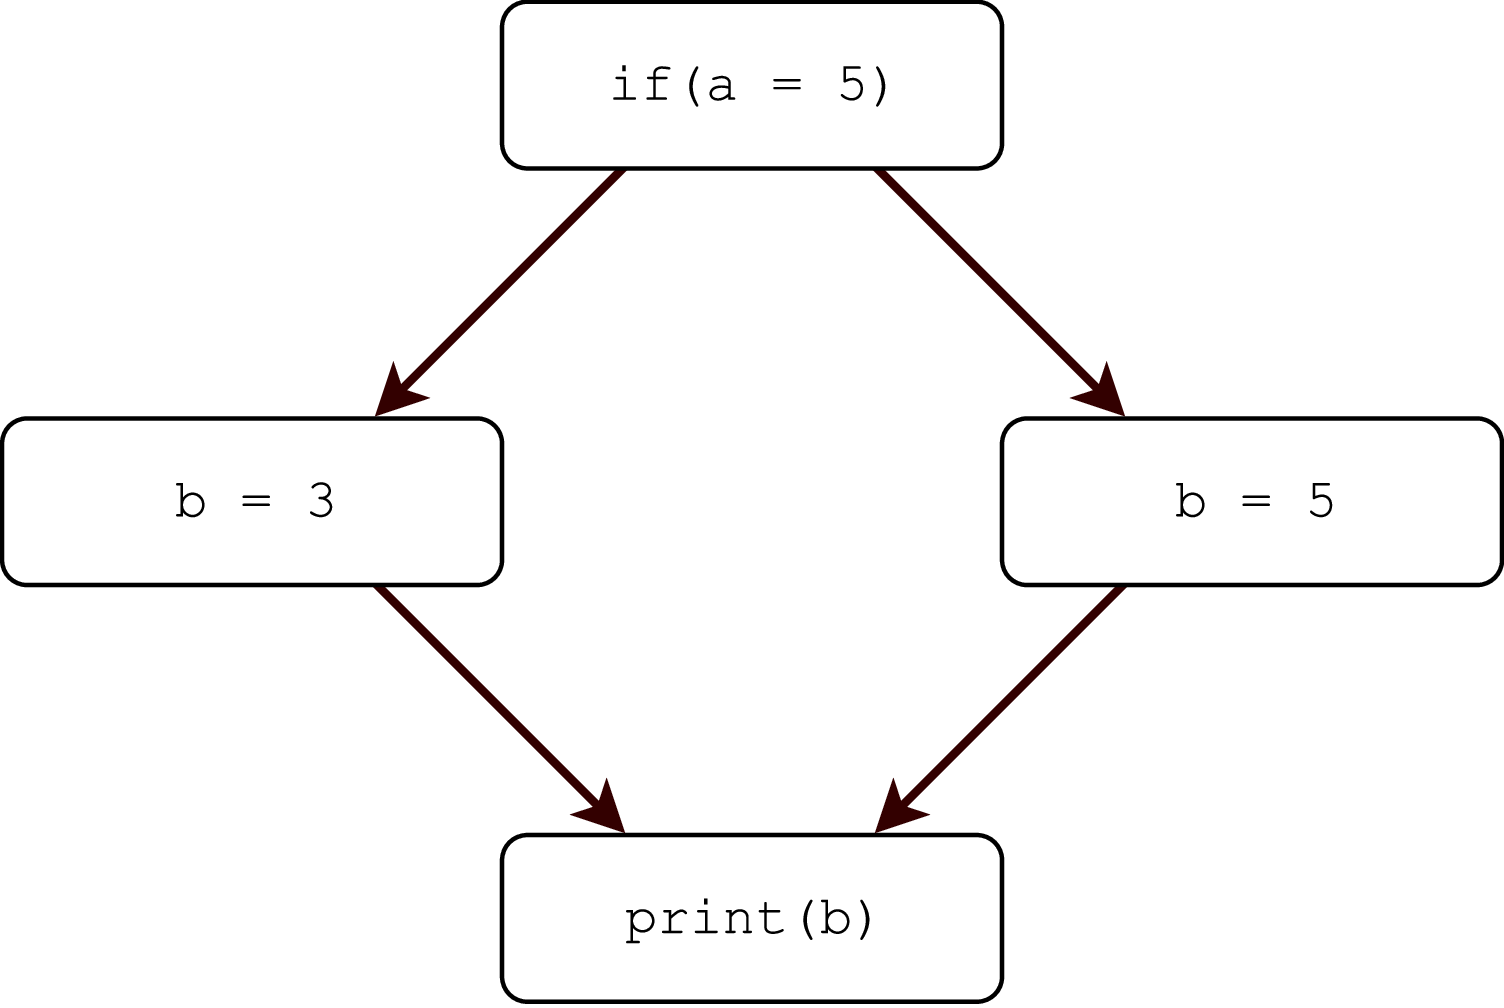
\includegraphics[width=\textwidth]{basic-cfg}
	\end{minipage}
\caption{Branching program and resulting CFG. Not in SSA form.}
\label{simple-cfg}
\end{figure}
\begin{figure}[t]
	\begin{minipage}{0.4\textwidth}
		\begin{lstlisting}[style=c]
if (a1 = 5)
	b1 = 3
else
	b2 = 5
b3 = phi(b1,b2)
print(b3)
		\end{lstlisting}
	\end{minipage}\hfill
	\begin{minipage} {0.45\textwidth}
		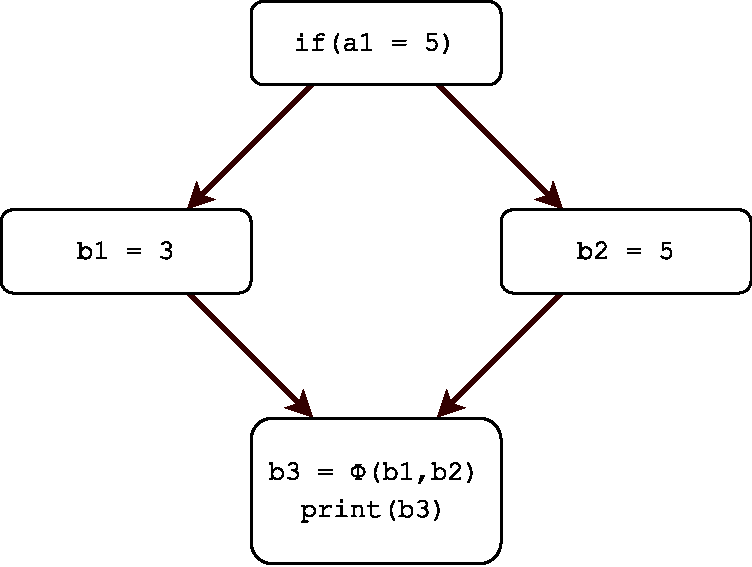
\includegraphics[width=\textwidth]{phi-node-simple}
	\end{minipage}
	\caption{Branching program and resulting CFG. Now in SSA form, with $\phi$-function resolving merging CFG paths}
	\label{simple-phi}
\end{figure}
\subsubsection{Def-Use and Use-Def Chains}
An important data structure in compiler analysis are def-use and use-def chains. The former is list of every use a definition has. Use-def chains point backwards to all definitions of variable, from the perspective of a use.  
\cite{Rastello:2016:SCD:3002539}

Due to the single definition variables of SSA, use-def chains are a single name, or element. Def-use chains can be build easily because they can be constructed through the single element use-def chains. We look at each use in the program and add the user to the definition's def-use list. Def-Use connections enable fast forward travelling through a CFG, because we are not bothered with code that is not part of the def-use chain. Figure \ref{def-use} shows an example of def-use connections for the variable \verb|a1|. The use-def connections would be the inversion of the dotted arrows. \cite{Rastello:2016:SCD:3002539}
\begin{figure}[t]
	\centering
	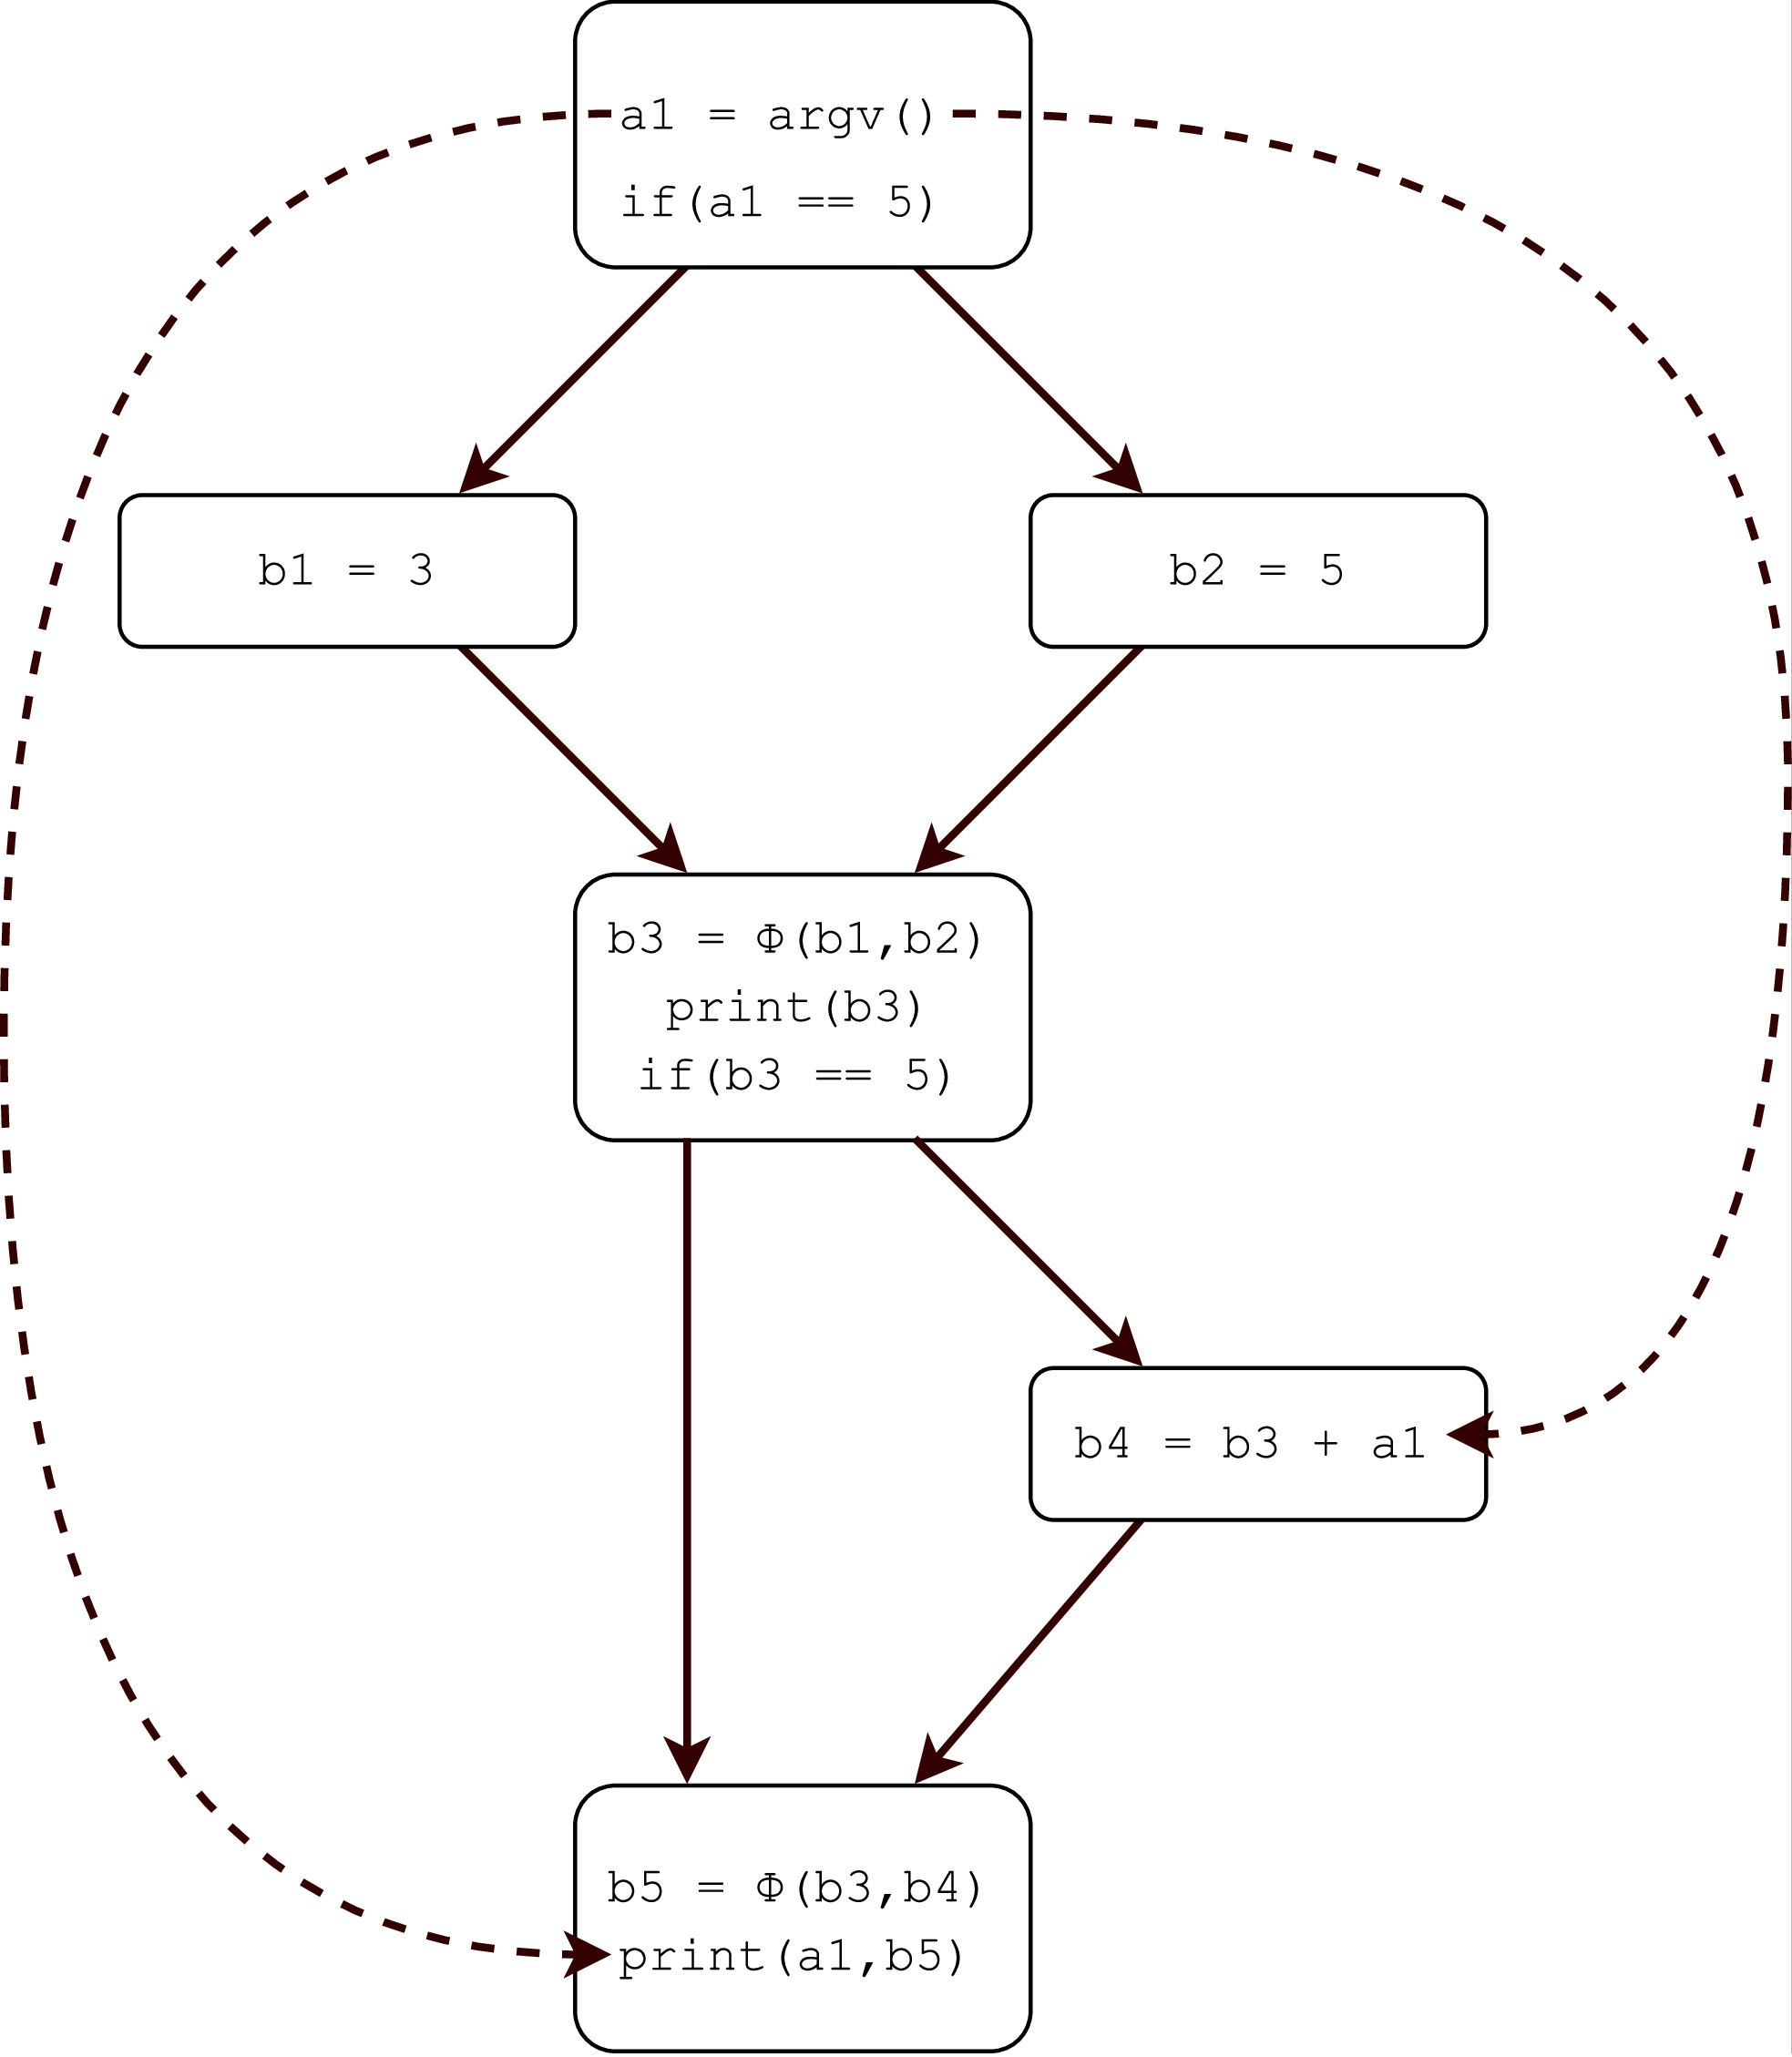
\includegraphics[width=0.6\textwidth]{def-use}
	\caption{Def-Use connections of variable a1 displayed as dotted lines.}
	\label{def-use}
\end{figure}

\subsection{LLVM Pass}\label{llvmpass}
A pass in LLVM is piece of software responsible for an analysis or transformation of IR. Passes are distinguished into said categories. An analysis pass creates or computer some information on the piece of IR it is running on, which later on can be used by other passes. It does modify the IR. As one pass may depend on the result of another analysis, passes are scheduled accordingly by the pass manager. A transformation pass alters the IR in place and does not produce any results. A transformation might trigger the re-run of an analysis as changes to the IR might invalidate the original results. Opposed to an analysis, transformations are not allowed to rely on results of other transformations. \cite{llvm-passes}
\subsubsection{Scopes}
A pass can run various scopes of IR. The pass can not access IR outside it's context and in the same pass, information can not be conveyed from one context to the next. For example: If a pass analyses functions, each function in the IR is analysed individually, with no knowledge about other functions. \cite{llvm-scopes}
\begin{itemize}
	\item \textbf{Module} scope contains the whole compilation unit with all it's functions and definitions. It is largest scope available.
	\item \textbf{Function} scope looks at every function individually. As the pass is limited to a function definition, it has no calling-context information. 
	\item \textbf{Loop} scope only provides access to the loop head and body, including loops nested into the loop.
	\item \textbf{BasicBlock} can only access a single basic-block. No CFG Manipulation possible.
\end{itemize}

\section{Compiler Techniques}
This section will briefly introduce terminology for two types of analysis and transformation a compiler can perform, which are relevant
for this work.
\subsection{Data Flow Analysis}
Data flow Analysis is a broad field, with some shared terminology that is described here. Generally, such an analysis traverses the code,
search for specific facts and optimizing the code according to the analysis results. Examples are constant propagation or zero value propagation. It is also closely related to pointer analysis, in terms of terminology and overall structure.
\begin{itemize}
	\item \textbf{Property Space} is a set of analysis facts. Represented as partially ordered sets with anti-symmetric, transitive and reflexive relation.\cite{Rastello:2016:SCD:3002539}
	\item A \textbf{Transfer function} classifies each visited analysis object, and determines to which set of the property space an object belongs to. To avoid loops, the transfer function needs to be monotonic. \cite{Rastello:2016:SCD:3002539}
	\item \textbf{Program Representation} is how the program is represented during the analysis. Usually, it is the CFG, but more sparse representation like def-use connections can be used as well. \cite{Rastello:2016:SCD:3002539}
	\item \textbf{Context Sensitive} describes the attribute, that the analysis of a function is sensitive to the context the function is called in. For example, the function
	takes the functions arguments into regard. \cite{Emami:1994:CIP:178243.178264}
	\item \textbf{Flow Sensitivity} defines that the sequence of instructions is importance for the analysis. \cite{Hardekopf:2009:SFP:1480881.1480911}
\end{itemize}

\subsection{Function Specialization}
Specialization (sometime procedure cloning) create distinct versions of a functions for a specific purpose at compile time. The technique was first introduced in \cite{Cooper:1993:MPC:2245763.2246020}. It resembles templates in C++, creating a function for every template used argument. A specialized function relies on information gathered during the analysis to optimize create a specialized version. An example for this are functions with differently unrolled loops, depending on the calling context of the function.

It differs from inlining, because it doesn't interfere with the original code structure and does not inflate the source code size. The difference to traditional data-flow analysis based optimizations is that it's possible to create multiple specialized versions for multiple data-flow facts, that vary depending on the calling context.   